\documentclass[12pt]{article}
\usepackage[left=1cm, right=1cm, top=2cm,bottom=1.5cm]{geometry} 

\usepackage[parfill]{parskip}
\usepackage[utf8]{inputenc}
\usepackage[T2A]{fontenc}
\usepackage[russian]{babel}
\usepackage{enumitem}
\usepackage[normalem]{ulem}
\usepackage{amsfonts, amsmath, amsthm, amssymb, mathtools,xcolor}
\usepackage{blkarray}

\usepackage{tabularx}
\usepackage{hhline}

\usepackage{accents}
\usepackage{fancyhdr}
\pagestyle{fancy}
\renewcommand{\headrulewidth}{1.5pt}
\renewcommand{\footrulewidth}{1pt}

\usepackage{graphicx}
\usepackage[figurename=Рис.]{caption}
\usepackage{subcaption}
\usepackage{float}

%%Наименование папки откуда забирать изображения
\graphicspath{ {./images/} }

%%Изменение формата для ввода доказательства
\renewcommand{\proofname}{$\square$  \nopunct}
\renewcommand\qedsymbol{$\blacksquare$}

%%Изменение отступа на таблицах
\addto\captionsrussian{%
	\renewcommand{\proofname}{$\square$ \nopunct}%
}
%% Римские цифры
\newcommand{\RN}[1]{%
	\textup{\uppercase\expandafter{\romannumeral#1}}%
}

%% Для удобства записи
\newcommand{\MR}{\mathbb{R}}
\newcommand{\MC}{\mathbb{C}}
\newcommand{\MQ}{\mathbb{Q}}
\newcommand{\MN}{\mathbb{N}}
\newcommand{\MZ}{\mathbb{Z}}
\newcommand{\MTB}{\mathbb{T}}
\newcommand{\MTI}{\mathbb{I}}
\newcommand{\MI}{\mathrm{I}}
\newcommand{\MCI}{\mathcal{I}}
\newcommand{\MJ}{\mathrm{J}}
\newcommand{\MH}{\mathrm{H}}
\newcommand{\MT}{\mathrm{T}}
\newcommand{\MU}{\mathcal{U}}
\newcommand{\MV}{\mathcal{V}}
\newcommand{\MB}{\mathcal{B}}
\newcommand{\MF}{\mathcal{F}}
\newcommand{\MW}{\mathcal{W}}
\newcommand{\ML}{\mathcal{L}}
\newcommand{\MP}{\mathcal{P}}
\newcommand{\VN}{\varnothing}
\newcommand{\VE}{\varepsilon}
\newcommand{\dx}{\, dx}
\newcommand{\dy}{\, dy}
\newcommand{\dz}{\, dz}
\newcommand{\dd}{\, d}


\theoremstyle{definition}
\newtheorem{defn}{Опр:}
\newtheorem{rem}{Rm:}
\newtheorem{prop}{Утв.}
\newtheorem{exrc}{Упр.}
\newtheorem{problem}{Задача}
\newtheorem{lemma}{Лемма}
\newtheorem{theorem}{Теорема}
\newtheorem{corollary}{Следствие}

\newenvironment{cusdefn}[1]
{\renewcommand\thedefn{#1}\defn}
{\enddefn}

\DeclareRobustCommand{\divby}{%
	\mathrel{\text{\vbox{\baselineskip.65ex\lineskiplimit0pt\hbox{.}\hbox{.}\hbox{.}}}}%
}
\DeclareRobustCommand{\ndivby}{\mkern-1mu\not\mathrel{\mkern4.5mu\divby}\mkern1mu}


%Короткий минус
\DeclareMathSymbol{\SMN}{\mathbin}{AMSa}{"39}
%Длинная шапка
\newcommand{\overbar}[1]{\mkern 1.5mu\overline{\mkern-1.5mu#1\mkern-1.5mu}\mkern 1.5mu}
%Функция знака
\DeclareMathOperator{\sgn}{sgn}

%Функция ранга
\DeclareMathOperator{\rk}{\text{rk}}
\DeclareMathOperator{\diam}{\text{diam}}


%Обозначение константы
\DeclareMathOperator{\const}{\text{const}}

\DeclareMathOperator{\codim}{\text{codim}}

\DeclareMathOperator*{\dsum}{\displaystyle\sum}
\newcommand{\ddsum}[2]{\displaystyle\sum\limits_{#1}^{#2}}
\newcommand{\ddssum}[2]{\displaystyle\smashoperator{\sum\limits_{#1}^{#2}}}
\newcommand{\ddlsum}[2]{\displaystyle\smashoperator[l]{\sum\limits_{#1}^{#2}}}
\newcommand{\ddrsum}[2]{\displaystyle\smashoperator[r]{\sum\limits_{#1}^{#2}}}

%Интеграл в большом формате
\DeclareMathOperator{\dint}{\displaystyle\int}
\newcommand{\ddint}[2]{\displaystyle\int\limits_{#1}^{#2}}
\newcommand{\ssum}[1]{\displaystyle \sum\limits_{n=1}^{\infty}{#1}_n}

\newcommand{\smallerrel}[1]{\mathrel{\mathpalette\smallerrelaux{#1}}}
\newcommand{\smallerrelaux}[2]{\raisebox{.1ex}{\scalebox{.75}{$#1#2$}}}

\newcommand{\smallin}{\smallerrel{\in}}
\newcommand{\smallnotin}{\smallerrel{\notin}}

\newcommand*{\medcap}{\mathbin{\scalebox{1.25}{\ensuremath{\cap}}}}%
\newcommand*{\medcup}{\mathbin{\scalebox{1.25}{\ensuremath{\cup}}}}%

\makeatletter
\newcommand{\vast}{\bBigg@{3.5}}
\newcommand{\Vast}{\bBigg@{5}}
\makeatother

%Промежуточное значение для sup\inf, поскольку они имеют разную высоту
\newcommand{\newsup}{\mathop{\smash{\mathrm{sup}}}}
\newcommand{\newinf}{\mathop{\mathrm{inf}\vphantom{\mathrm{sup}}}}

%Скалярное произведение
\newcommand{\inner}[2]{\left\langle #1, #2 \right\rangle }
\newcommand{\linsp}[1]{\left\langle #1 \right\rangle }
\newcommand{\linmer}[2]{\left\langle #1 \vert #2\right\rangle }

%Подпись символов снизу
\newcommand{\ubar}[1]{\underaccent{\bar}{#1}}

%%Шапка для букв сверху
\newcommand{\wte}[1]{\widetilde{#1}}
\newcommand{\wht}[1]{\widehat{#1}}
\newcommand{\ovl}[1]{\overline{#1}}


%%Трансформация Фурье
\newcommand{\fourt}[1]{\mathcal{F}\left(#1\right)}
\newcommand{\ifourt}[1]{\mathcal{F}^{-1}\left(#1\right)}

%%Символ вектора
\newcommand{\vecm}[1]{\overrightarrow{#1\,}}

%%Пространстов матриц
\newcommand{\matsq}[1]{\operatorname{Mat}_{#1}}
\newcommand{\mat}[2]{\operatorname{Mat}_{#1, #2}}

%Оператор для действ и мнимых чисел
\DeclareMathOperator{\IM}{\operatorname{Im}}
\DeclareMathOperator{\RE}{\operatorname{Re}}
\DeclareMathOperator{\li}{\operatorname{li}}
\DeclareMathOperator{\GL}{\operatorname{GL}}
\DeclareMathOperator{\SL}{\operatorname{SL}}
\DeclareMathOperator{\Char}{\operatorname{char}}
\DeclareMathOperator\Arg{Arg}
\DeclareMathOperator\ord{ord}

%Оператор для образа
\DeclareMathOperator{\Ima}{Im}

%Делимость чисел
\newcommand{\modn}[3]{#1 \equiv #2 \; (\bmod \; #3)}
\newcommand{\nmodn}[3]{#1 \not\equiv #2 \; (\bmod \; #3)}

%%Взятие в скобки, модули и норму
\newcommand{\parfit}[1]{\left( #1 \right)}
\newcommand{\modfit}[1]{\left| #1 \right|}
\newcommand{\sqparfit}[1]{\left\{ #1 \right\}}
\newcommand{\normfit}[1]{\left\| #1 \right\|}

%%Функция для обозначения равномерной сходимости по множеству
\newcommand{\uconv}[1]{\overset{#1}{\rightrightarrows}}
\newcommand{\uconvm}[2]{\overset{#1}{\underset{#2}{\rightrightarrows}}}


%%Функция для обозначения нижнего и верхнего интегралов
\def\upint{\mathchoice%
	{\mkern13mu\overline{\vphantom{\intop}\mkern7mu}\mkern-20mu}%
	{\mkern7mu\overline{\vphantom{\intop}\mkern7mu}\mkern-14mu}%
	{\mkern7mu\overline{\vphantom{\intop}\mkern7mu}\mkern-14mu}%
	{\mkern7mu\overline{\vphantom{\intop}\mkern7mu}\mkern-14mu}%
	\int}
\def\lowint{\mkern3mu\underline{\vphantom{\intop}\mkern7mu}\mkern-10mu\int}

%%След матрицы
\DeclareMathOperator*{\tr}{tr}

\makeatletter
\renewcommand*\env@matrix[1][*\c@MaxMatrixCols c]{%
	\hskip -\arraycolsep
	\let\@ifnextchar\new@ifnextchar
	\array{#1}}
\makeatother


%% Переопределение функции хи, чтобы выглядела более приятно
\makeatletter
\@ifdefinable\@latex@chi{\let\@latex@chi\chi}
\renewcommand*\chi{{\@latex@chi\smash[t]{\mathstrut}}} % want only bottom half of \mathstrut
\makeatletter

\setcounter{MaxMatrixCols}{20}

\begin{document}
\lhead{Математический анализ - \RN{4}}
\chead{Шапошников С.В.}
\rhead{Лекция - 1}
\section*{Интеграл Римана в $\MR^n$}

\subsection*{Разбиения в $\MR^n$}
Рассмотрим пространство $\MR^n$.
\begin{defn}
	Пусть $\MJ_1,\dotsc, \MJ_n \subset \MR$ - ограниченные промежутки: 
	$$
		(\alpha,\beta), (\alpha,\beta], [\alpha, \beta), [\alpha,\beta]
	$$
	Будем называть множество $\MI = \MJ_1 \times \MJ_2 \times \dotsc \times \MJ_n$ \uwave{параллелепипидом} или \uwave{брусом}. 
\end{defn}

\begin{rem}
	Заметим, что этот объект называют брусом, поскольку параллелепипид это не обязательно такой объект, а здесь важно, что ребра этого параллелепипида параллельны осям координат.
\end{rem}
\begin{rem}
	Заметим также, что естественное обобщение отрезка на $\MR^n$ это брус. 
\end{rem}

\begin{figure}[H]
	\centering
	\includegraphics[width=0.25\textwidth]{MA4L1_1.eps}
	\caption{Пример бруса в $\MR^2$.}
	\label{4_1}
\end{figure}
\begin{defn}
	Брус $\MI = \MJ_1 \times \MJ_2 \times \dotsc \times \MJ_n$ называется \uwave{замкнутым}, если все $\MJ_k$ - это отрезки, то есть это декартово произведение отрезков.
\end{defn}

\begin{defn}
	\uwave{Объемом бруса} $\MI = \MJ_1 \times \dotsc \times \MJ_n$ назовём число: $|\MI| = |\MJ_1|{\cdot}\dotsc{\cdot}|\MJ_n|$. 
\end{defn}

Пусть $\MI$ - замкнутый брус, $\MI = [a_1,b_1]\times \dotsc \times [a_n,b_n]$. Возьмем разбиение каждого из отрезков: 
$$
	a_1 = x_1^0 < x_1^1 < \dotsc < x_1^{m_1} = b_1, \dotsc , a_n = x_n^0 < \dotsc < x_n^{m_n} = b_n
$$
Припишем этим разбиениям отрезки: $\Delta_i^k = \left[x_i^{k-1}, x_i^k\right], \, |\Delta_i^k| = x_i^{k} - x_i^{k-1}$. Если мы возьмем декартовые произведения всевозможных отрезков, то мы получим набор брусков:
$$
	\MI_{k_1\dotsc k_n} = \Delta_1^{k_1}\times \dotsc \times \Delta_n^{k_n}
$$ 
\begin{figure}[H]
	\centering
	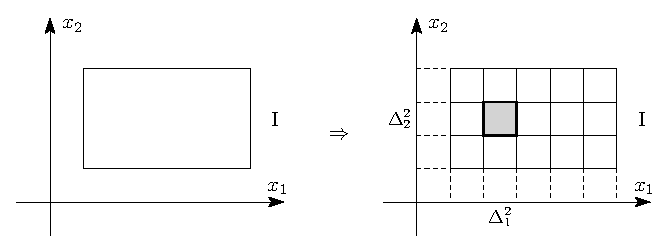
\includegraphics[width=0.7\textwidth]{MA4L1_2.eps}
	\caption{Пример разбиения бруса в $\MR^2$, брусок $\MI_{22}$.}
	\label{4_2}
\end{figure}
\begin{defn}
	\uwave{Разбиением бруска} $\MI$ назовем набор из брусков: $\MI_{k_1\dotsc k_n} = \Delta_1^{k_1}\times \dotsc \times \Delta_n^{k_n}$ и обозначим: $\MTB = \{\MI_m\}$.
\end{defn}
\begin{rem}
	Разбиение не обязательно должно быть таким, но в таком виде оно упрощает дальнейший разбор теории. Отметим, что клеточная структура общности не уменьшает.
\end{rem}

\begin{prop}
	Если $\{\MI_m\}$ - разбиение бруска $\MI$, то $|\MI| = \ddsum{k_1\dotsc k_n}{}|\MI_{k_1\dotsc k_n}|$.
\end{prop}
\begin{proof}
	По определению:
	$$
		|\MI| = \left(\left|\Delta_1^1\right| + \dotsc + \left|\Delta_1^{m_1}\right|\right){\cdot}\left(\left|\Delta_2^1\right| + \dotsc + \left|\Delta_2^{m_2}\right|\right){\cdot} \dotsc {\cdot} \left(\left|\Delta_n^1\right| + \dotsc + \left|\Delta_n^{m_n}\right|\right)
	$$  
	Раскроем скобки:
	$$
		|\MI| = \ddsum{k_1 \dotsc k_n}{}\left|\Delta_1^{k_1}\right|{\cdot}\dotsc{\cdot}\left|\Delta_n^{k_n}\right| = \ddsum{k_1 \dotsc k_n}{}|\MI_{k_1 \dotsc k_n}|
	$$
\end{proof}

\begin{defn}
	\uwave{Отмеченным разбиением} бруска $\MI$ назовем набор пар: 
	$$
		(\MTB,\xi) = \{(\MI_j,\xi_j) \mid \xi_j \in \MI_j \}
	$$
\end{defn}
\begin{defn}
	\uwave{Диаметром бруска} разбиения назовем максимальное расстояние между точками в бруске: 
	$$
		\diam{(\MI_m)} = d(\MI_m) = \sup\limits_{x,y \in \MI_m}\|x - y\|
	$$
\end{defn}
\begin{rem}
	У прямоугольника диаметром является длина диагонали.
\end{rem}
\begin{defn}
	\uwave{Масштабом разбиения} или \uwave{параметром разбиения} назовем максимум из всех диаметров брусков разбиения: 
	$$
		\lambda(\MTB) = \max\limits_{j}d(\MI_j)
	$$
\end{defn}
\subsection*{Интеграл Римана в $\MR^n$}
Пусть определена функция $f \colon \MI \to \MR$. 
\begin{defn}
	\uwave{Суммой Римана} называется следующее выражение:
	$$
		\sigma(f,\MTB,\xi) = \ddsum{j}{}f(\xi_j){\cdot}|\MI_j|
	$$
\end{defn}
\begin{figure}[H]
	\centering
	\includegraphics[width=0.45\textwidth]{MA4L1_3.png}
	\caption{Сумма Римана как ``объем'' под графиком $f$ над брусом $\MI$.}
	\label{4_3}
\end{figure}

\begin{defn}
	Число $A$ называется \uwave{интегралом Римана} функции $f$ по брусу $\MI$ ($f$ называется \uwave{интегрируемой по Риману} на $\MI$), если:
	$$
		\forall \VE > 0, \, \exists \, \delta > 0 \colon \forall (\MTB,\xi), \, \lambda(\MTB) < \delta \Rightarrow |\sigma(f,\MTB,\xi) - A| < \VE
	$$
	то есть, это предел по базе:
	$$
		\lim\limits_{\lambda(\MTB) \to 0} \sigma(f,\MTB,\xi) = A
	$$
	\textbf{\uline{Обозначение}}:
	$$
		A = \ddint{\MI}{}f(x)dx = \ddint{\MI}{}f(x_1,\dotsc, x_n)dx_1\dotsc dx_n =  \int\idotsint\limits_{\MI} f(x_1,\dotsc, x_n)dx_1\dotsc dx_n 
	$$
\end{defn}
\begin{prop}(\textbf{простейшие свойства интеграла})
	\begin{enumerate}[label=\arabic*)]
		\item Если $f$ интегрируема на $\MI$, то $f$ ограничена;
		\item Если $f,g$ интегрируемы на $\MI$, то $\forall \alpha,\beta \in \MR,\, \alpha f+ \beta g$ интегрируема на $\MI$ и верно:
		$$
			\ddint{\MI}{}(\alpha f(x) + \beta g(x))dx = \alpha \ddint{\MI}{}f(x)dx + \beta \ddint{\MI}{}g(x)dx
		$$
		\item Если $f,g$ интегрируемы на $\MI$ и $f(x) \leq g(x)$, то верно:
		$$
			\ddint{\MI}{}f(x)dx \leq \ddint{\MI}{}g(x)dx
		$$
	\end{enumerate}
\end{prop}
\begin{proof}\hfill
	\begin{enumerate}[label=\arabic*)]
		\item Пусть $A$ это интеграл $f$, возьмем $\VE = 1$, тогда: $\exists \, \delta > 0 \colon \forall (\MTB,\xi), \, \lambda(\MTB)  < \delta$ такое, что будет верно:
		$$
			A - \VE < \ddsum{j}{}f(\xi_j){\cdot}|\MI_j| < A + \VE
		$$
		Заметим, что $|\MI_j| > 0$ и $\xi_j$ - произвольная точка из $\MI_j$. Докажем от противного. Пусть $f$ не является ограниченной $\Rightarrow \exists\, k \colon f$ не является ограниченной на бруске $\MI_k$. Фиксируем $\xi_j, \, \forall j \neq k$ и переписываем неравенство:
		$$
			\const = A - \VE - \ddsum{j \neq k}{}f(\xi_j){\cdot}|\MI_j| < f(\xi_k){\cdot}|\MI_k| < A + \VE - \ddsum{j \neq k}{}f(\xi_j){\cdot}|\MI_j| = \const
		$$
		$$
			|\MI_j| = \const \neq 0 \Rightarrow |f(\xi_j)| < \infty
		$$
		$f(\xi_k)$ - ограниченно, но $\xi_k$ - произвольное $\Rightarrow f(x)$ ограниченно на $\MI_k \Rightarrow$ противоречие;
		\item По линейности суммы: $\sigma(\alpha f + \beta g, \MTB, \xi) = \alpha\sigma(f,\MTB,\xi) + \beta\sigma(g,\MTB,\xi)$. Рассмотрим сразу $\delta > 0$ общее для $f$ и $g$ (минимум из $\delta_f, \, \delta_g$) так, чтобы:
		$$
			\left|\ddint{\MI}{}f(x)dx - \sigma(f,\MTB,\xi)\right| < \VE \wedge 	\left|\ddint{\MI}{}g(x)dx - \sigma(g,\MTB,\xi)\right| < \VE
		$$
		По неравенству треугольника:
		$$
			\left|\ddint{\MI}{}(\alpha f(x) + \beta g(x))dx - \sigma(\alpha f + \beta g, \MTB, \xi)\right| \leq |\alpha|{\cdot}\left|\ddint{\MI}{}f(x)dx - \sigma(f, \MTB,\xi)\right| + 
		$$
		$$
			+|\beta|{\cdot}\left|\ddint{\MI}{}g(x)dx - \sigma(g,\MTB,\xi)\right| \leq ( |\alpha| + |\beta|)\VE
		$$
		\item По линейности достаточно доказать, что $f \geq 0 \Rightarrow A = \ddint{\MI}{}f(x)dx \geq 0$. По определению:
		$$
			\forall \VE > 0, \, \exists \, \delta > 0 \colon \forall (\MTB,\xi), \, \lambda(\MTB) < \delta \Rightarrow A + \VE \geq \sigma(f,\MTB,\xi) = \ddsum{j}{}f(\xi_j){\cdot}|\MI_j| \geq 0  \Rightarrow
		$$
		$$
			\Rightarrow A \geq -\VE \Rightarrow \lim\limits_{\VE \to 0}A \geq \lim\limits_{\VE \to 0}(-\VE) =0  \Rightarrow A \geq 0
		$$
	\end{enumerate}
\end{proof}

\subsection*{Характеристическая функция}
\begin{defn}
	Пусть $\MI$ - замкнутый брус и $\MJ \subset \MI$ - произвольный брус. Функция вида: 
	$$
		\chi_{\MJ}(x) = 
		\begin{cases}
			1, & x \in \MJ\\
			0, & x \not\in \MJ
		\end{cases}
	$$
	называется \uwave{характеристической функцией}.
\end{defn}

\begin{figure}[H]
	\centering
	\includegraphics[width=0.22\textwidth]{MA4L1_4.eps}
	\caption{Характеристическая функция $\chi_{\MJ}(x)$.}
	\label{4_4}
\end{figure}
Распишем подробнее: $\MJ = \MJ_1\times \dotsc \times \MJ_n \Rightarrow \chi_{\MJ}(x) = \chi_{\MJ_1}(x_1){\cdot}\dotsc{\cdot}\chi_{\MJ_n}(x_n)$, поскольку лежать в декартовом произведении означает, что каждая координата лежит в нужной части декартового произведения. Таким образом, мы получаем единицу только в том случае, когда весь набор $(x_1,\dotsc, x_n)$ лежит в $\MJ$.

\begin{prop}
	$\ddint{\MI}{}\chi_{\MJ}(x) dx = |\MJ|$.
\end{prop}
\begin{proof}
	При $n = 1$ уже доказано (см. семестр $2$, лекция $21$). Пусть $(\MTB,\xi)$ - отмеченное разбиение, $\MTB$ будет устроено следующим образом:
	$$
		\MTB = \left\{\MI_{k_1\dotsc k_n}, \, \xi^\varkappa = (\xi_1^{\varkappa}, \dotsc, \xi_n^{\varkappa})\right\}, \, \MI_{k_1 \dotsc k_n} = \Delta_1^{k_1}\times \dotsc \times \Delta_n^{k_n}, \, \varkappa = (k_1\dotsc k_n)
	$$
	где $\xi^{\varkappa}$ означает, что для каждой клетки у нас есть своя отмеченная точка и координаты не обязаны совпадать между собой на одинаковых отрезках (выбор координаты зависит от всего набора индексов): 
	$$
		\varkappa' =(k_1,k'_2, \dotsc,k'_n) \neq \varkappa = (k_1, k_2, \dotsc, k_n) \Rightarrow \xi_1^{\varkappa} \neq \xi_1^{\varkappa'}, \, \xi_1^{\varkappa}, \xi_1^{\varkappa'} \in \Delta_1^{k_1}
	$$ 
	Рассмотрим Риманову сумму:
	$$
		\ddsum{\varkappa}{}\chi_{\MJ}(\xi^{\varkappa}){\cdot}|\MI_{\varkappa}| = \ddsum{k_1 \dotsc k_n}{}\chi_{\MJ_1}(\xi_1^{\varkappa}){\cdot}\dotsc{\cdot}\chi_{\MJ_n}(\xi_n^{\varkappa}){\cdot}|\Delta_1^{k_1}|{\cdot}\dotsc{\cdot}|\Delta_n^{k_n}|, \quad \xi_1^{\varkappa} \in \Delta_1^{k_1}, \dotsc, \xi_n^{\varkappa} \in \Delta_n^{k_n} \Rightarrow
	$$
	$$
		\Rightarrow \ddsum{k_1 \dotsc k_n}{}\chi_{\MJ_1}(\xi_1^{\varkappa}){\cdot}\dotsc{\cdot}\chi_{\MJ_n}(\xi_n^{\varkappa}){\cdot}|\Delta_1^{k_1}|{\cdot}\dotsc{\cdot}|\Delta_n^{k_n}| \leq \ddsum{k_1 \dotsc k_n}{} \sup\limits_{x_1 \smallin \Delta_1^{k_1}}\chi_{\MJ_1}(x_1){\cdot}\dotsc{\cdot}\sup\limits_{x_n \smallin\Delta_n^{k_n}}\chi_{\MJ_n}(x_n){\cdot}|\Delta_1^{k_1}|{\cdot}\dotsc{\cdot}|\Delta_n^{k_n}| = 
	$$
	$$
		= \left(\ddsum{k_1}{}\sup\limits_{x_1 \smallin \Delta_1^{k_1}}\chi_{\MJ_1}(x_1){\cdot}|\Delta_1^{k_1}|\right){\cdot}\dotsc{\cdot}\left(\ddsum{k_n}{}\sup\limits_{x_n \smallin \Delta_n^{k_n}}\chi_{\MJ_n}(x_n){\cdot}|\Delta_n^{k_n}|\right)
	$$
	В скобочках записаны одномерные верхние суммы Дарбу. Заметим, что:
	$$
		\lambda(\MTB) \to 0 \Rightarrow \max\limits_{k_1}|\Delta_1^{k_1}|\to 0, \dotsc, \max\limits_{k_n}|\Delta_n^{k_n}| \to 0
	$$
	Тогда:
	$$
		\lim\limits_{\lambda(\MTB)\to 0}\left(\ddsum{k_1}{}\sup\limits_{x_1 \smallin \Delta_1^{k_1}}\chi_{\MJ_1}(x_1){\cdot}|\Delta_1^{k_1}|\right){\cdot}\dotsc{\cdot}\left(\ddsum{k_n}{}\sup\limits_{x_n \smallin\Delta_n^{k_n}}\chi_{\MJ_n}(x_n){\cdot}|\Delta_n^{k_n}|\right) = 
	$$
	$$
		= \left(\ddint{a_1}{b_1}\chi_{\MJ_1}(x_1)dx_1 \right){\cdot}\dotsc{\cdot}\left(\ddint{a_n}{b_n}\chi_{\MJ_n}(x_n)dx_n \right) = |\MJ_1|{\cdot}\dotsc{\cdot}|\MJ_n| = |\MJ|
	$$
	По аналогии, оценим снизу:
	$$
		\ddsum{\varkappa}{}\chi_\MJ(\xi^{\varkappa}){\cdot}|\MI_{\varkappa}| \geq \left(\ddsum{k_1}{}\inf_{x_1 \smallin \Delta_1^{k_1}}\chi_{\MJ_1}(x_1){\cdot}|\Delta_1^{k_1}|\right){\cdot} \dotsc {\cdot}\left(\ddsum{k_n}{}\inf_{x_n \smallin\Delta_n^{k_n}}\chi_{\MJ_n}(x_n){\cdot}|\Delta_n^{k_n}|\right) \Rightarrow 
	$$
	$$	
		\Rightarrow \lim\limits_{\lambda(\MTB)\to 0} \left(\ddsum{k_1}{}\inf_{x_1 \smallin \Delta_1^{k_1}}\chi_{\MJ_1}(x_1){\cdot}|\Delta_1^{k_1}|\right){\cdot} \dotsc {\cdot}\left(\ddsum{k_n}{}\inf_{x_n \smallin\Delta_n^{k_n}}\chi_{\MJ_n}(x_n){\cdot}|\Delta_n^{k_n}|\right) =
	$$
	$$
		= \left(\ddint{a_1}{b_1}\chi_{\MJ_1}(x_1)dx_1 \right){\cdot}\dotsc{\cdot}\left(\ddint{a_n}{b_n}\chi_{\MJ_n}(x_n)dx_n \right) =  |\MJ_1|{\cdot}\dotsc{\cdot}|\MJ_n| = |\MJ|
	$$
	Следовательно: $\sigma\left(\chi_{\MJ},\MTB,\xi\right) \xrightarrow[\lambda(\MTB) \to 0]{} |\MJ|$.
\end{proof}
\begin{exrc}
	Пусть $f_1,\dotsc, f_n \geq 0$ и $f_k$ интегрируемы на $[a_k,b_k]$, $\MI = [a_1,b_1]\times \dotsc \times [a_n,b_n]$. Доказать, что $f_1(x_1){\cdot}\dotsc{\cdot}f_n(x_n)$ - интегрируема на $\MI$ и верно:
	$$
		\ddint{\MI}{}f_1(x_1){\cdot}\dotsc{\cdot} f_n(x_n)dx_1 \dotsc dx_n = \ddint{a_1}{b_1}f_1(x_1)dx_1{\cdot}\dotsc{\cdot}\ddint{a_n}{b_n}f_n(x_n)dx_n
	$$
\end{exrc}
\begin{proof}
	Доказательство проводится по полной аналогии с предыдущей задачей. Пусть начальные условия такие же. Введём обозначение:
	$$
		f(x) = f_1(x_1){\cdot}\dotsc{\cdot}f_n(x_n), \, \forall x = (x_1,\dotsc,x_n) \in \MI
	$$
	Рассмотрим Римановы суммы (с учётом того, что $\forall i = \overline{1,n}, \, f_i \geq 0$):
	$$
		\ddsum{\varkappa}{}f(\xi^{\varkappa}){\cdot}|\MI_{\varkappa}| = \ddsum{k_1 \dotsc k_n}{}f_1(\xi_1^{\varkappa}){\cdot}\dotsc{\cdot}f_n(\xi_n^{\varkappa}){\cdot}|\Delta_1^{k_1}|{\cdot}\dotsc{\cdot}|\Delta_n^{k_n}|, \quad \xi_1^{\varkappa} \in \Delta_1^{k_1}, \dotsc, \xi_n^{\varkappa} \in \Delta_n^{k_n} \Rightarrow
	$$
	$$
		\Rightarrow \ddsum{k_1 \dotsc k_n}{}f_1(\xi_1^{\varkappa}){\cdot}\dotsc{\cdot}f_n(\xi_n^{\varkappa}){\cdot}|\Delta_1^{k_1}|{\cdot}\dotsc{\cdot}|\Delta_n^{k_n}| \leq \ddsum{k_1 \dotsc k_n}{} \sup\limits_{x_1 \smallin \Delta_1^{k_1}}f_1(x_1){\cdot}\dotsc{\cdot}\sup\limits_{x_n \smallin\Delta_n^{k_n}}f_n(x_n){\cdot}|\Delta_1^{k_1}|{\cdot}\dotsc{\cdot}|\Delta_n^{k_n}| = 
	$$
	$$
		= \left(\ddsum{k_1}{}\sup\limits_{x_1 \smallin \Delta_1^{k_1}}f_1(x_1){\cdot}|\Delta_1^{k_1}|\right){\cdot}\dotsc{\cdot}\left(\ddsum{k_n}{}\sup\limits_{x_n \smallin \Delta_n^{k_n}}f_n(x_n){\cdot}|\Delta_n^{k_n}|\right) \xrightarrow[\lambda(\MTB) \to 0]{} \left(\ddint{a_1}{b_1}f_1(x_1)dx_1 \right){\cdot}\dotsc{\cdot}\left(\ddint{a_n}{b_n}f_n(x_n)dx_n \right)
	$$
	По аналогии, оценим снизу:
	$$
		\ddsum{\varkappa}{}f(\xi^{\varkappa}){\cdot}|\MI_{\varkappa}| \geq \left(\ddsum{k_1}{}\inf_{x_1 \smallin \Delta_1^{k_1}}f_1(x_1){\cdot}|\Delta_1^{k_1}|\right){\cdot} \dotsc {\cdot}\left(\ddsum{k_n}{}\inf_{x_n \smallin\Delta_n^{k_n}}f_n(x_n){\cdot}|\Delta_n^{k_n}|\right) \Rightarrow 
	$$
	$$	
		\Rightarrow \lim\limits_{\lambda(\MTB)\to 0} \left(\ddsum{k_1}{}\inf_{x_1 \smallin \Delta_1^{k_1}}f_1(x_1){\cdot}|\Delta_1^{k_1}|\right){\cdot} \dotsc {\cdot}\left(\ddsum{k_n}{}\inf_{x_n \smallin\Delta_n^{k_n}}f_n(x_n){\cdot}|\Delta_n^{k_n}|\right) = \left(\ddint{a_1}{b_1}f_1(x_1)dx_1 \right){\cdot}\dotsc{\cdot}\left(\ddint{a_n}{b_n}f_n(x_n)dx_n \right)
	$$
	Следовательно: 
	$$
		\sigma\left(f,\MTB,\xi\right) \xrightarrow[\lambda(\MTB) \to 0]{} \ddint{\MI}{}f_1(x_1){\cdot}\dotsc{\cdot} f_n(x_n)dx_1 \dotsc dx_n = \ddint{a_1}{b_1}f_1(x_1)dx_1{\cdot}\dotsc{\cdot}\ddint{a_n}{b_n}f_n(x_n)dx_n
	$$
\end{proof}

\textbf{Пример}: Рассмотрим неинтегрируемую функцию: 
$$
	D(s) = \begin{cases}
		1, & s \in \MQ \\
		0, & s \not\in \MQ
	\end{cases}
$$
это функция Дирихле и рассмотрим произведение этих функций: $\wte{D}(x) = D(x_1){\cdot}\dotsc{\cdot}D(x_n)$. Эта функция не является интегрируемой на всяком брусе $\MI$. Выбирая отмеченные точки сумма Римана может принимать два значения:
$$
	\sigma\left(\wte{D},\MTB,\xi\right) = \begin{cases}
		|\MI|, & \xi \in \MQ^n\\
		0, & \xi \not\in \MQ^n
	\end{cases}
$$
Сумма Римана не зависит от $\lambda(\MTB) \Rightarrow$ нет сходимости $\Rightarrow$ функция не интегрируема.

\begin{defn}
	Пусть $\MI$ - замкнутый брус. $\{\MJ_m\}$ - произвольный набор брусков в $\MI, \, m = \overline{1,M}$. Функцию вида:
	$$
		f(x) = \ddsum{m = 1}{M}c_m \chi_{\MJ_m}(x)
	$$
	будем называть \uwave{ступенчатой функцией}.
\end{defn}
\begin{corollary}
	Ступенчатая функция $f$ интегрируема на $\MI$ и верно равенство:
	$$
		\ddint{\MI}{}f(x) dx = \ddsum{m = 1}{M}c_m{\cdot}|\MJ_m|
	$$
\end{corollary}
\begin{proof}
	Сразу следует из линейности интеграла и утверждения про интеграл функции $\chi_{\MJ}(x)$ выше.
\end{proof}

\begin{corollary}
	Пусть $\MJ, \MJ_1,\dotsc, \MJ_M$ - бруски и брусок $\MJ \subset \displaystyle\bigcup\limits_{m = 1}^{M}\MJ_m$, тогда: 
	$$
		|\MJ| \leq \ddsum{m = 1}{M}|\MJ_m|
	$$
\end{corollary}
\begin{proof}
	Очевидно, что $\chi_{\MJ} \leq \ddsum{m = 1}{M}\chi_{\MJ_m}$, поскольку на каждой точке из $\MJ$ справа будет хотя бы одна единица. Возьмем брус $\MI$, который содержит все данные бруски. Тогда по линейности и монотонности:
	$$
		|\MJ| = \ddint{\MI}{}\chi_{\MJ}(x)dx \leq \ddint{\MI}{}\ddsum{m = 1}{M}\chi_{\MJ_m}(x)dx = \ddsum{m = 1}{M}\ddint{\MI}{}\chi_{\MJ_m}(x)dx = \ddsum{m = 1}{M}|\MJ_m|
	$$
\end{proof}
\begin{exrc}
	Пусть $\MJ = \displaystyle \bigcup\limits_{m = 1}^{M}\MJ_m$ и $\MJ_m \cap \MJ_l = \VN, \, \forall m \neq l$. Доказать, что: $|\MJ| = \ddsum{m = 1}{M}|\MJ_m|$.
\end{exrc}
\begin{proof}
	$$
		x \in \MJ \Leftrightarrow \exists \, k =\ovl{1,n} \colon x \in \MJ_k \Rightarrow \forall x \in \MJ, \, \chi_\MJ(x) = \ddsum{m = 1}{M}\chi_{\MJ_m}(x)
	$$
	Возьмем брус $\MI$, который содержит все данные бруски. Тогда по линейности:
	$$
		|\MJ| = \ddint{\MI}{}\chi_{\MJ}(x)dx = \ddint{\MI}{}\ddsum{m = 1}{M}\chi_{\MJ_m}(x)dx = \ddsum{m = 1}{M}\ddint{\MI}{}\chi_{\MJ_m}(x)dx = \ddsum{m = 1}{M}|\MJ_m|
	$$
\end{proof}
\begin{rem}
	Если бруски пересекаются только по граням, тогда:
	$$
		\forall x\in \MJ, \, \chi_{\MJ}(x) = \ddsum{m = 1}{M}\chi_{\wht{\MJ}_m}(x) + \ddsum{k < l}{}\chi_{\MJ_k \cap \MJ_l}(x)
	$$
	где $\forall m \neq l,\, \wht{\MJ}_m \cap \wht{\MJ}_l = \VN$, а пересечение возможно лишь по граням. В этом случае, по аддитивности:
	$$
		|\MJ| = \ddint{\MI}{}\chi_{\MJ}(x)dx = \ddint{\MI}{}\left(\ddsum{m = 1}{M}\chi_{\wht{\MJ}_m}(x) + \ddsum{k < l}{}\chi_{\MJ_k \cap \MJ_l}(x)\right)dx = \ddsum{m = 1}{M}\ddint{\MI}{}\chi_{\wht{\MJ}_m}(x)dx + 0  = \ddsum{m = 1}{M}|\MJ_m|
	$$
\end{rem}


\section*{Перестановка интеграла и предела}
\begin{prop}
	Пусть $f$ - интегрируема на брусе $\MI$, тогда верно равенство:
	$$
		\left|\ddint{\MI}{}f(x)dx \right| \leq \sup\limits_{\MI}{|f|}{\cdot}|\MI| 
	$$
\end{prop}
\begin{proof}
	Очевидно, что: 
	$$
			-\sup\limits_{\MI}|f|{\cdot}\chi_{\MI}(x) \leq f(x) \leq \sup\limits_{\MI}|f|{\cdot}\chi_{\MI}(x)   
	$$
	Воспользуемся свойством монотонности и линейности:
	$$
			-\sup\limits_{\MI}|f|{\cdot}|\MI| \leq \ddint{\MI}{}f(x)dx \leq \sup\limits_{\MI}|f|{\cdot}|\MI|
	$$
\end{proof}
\begin{theorem}
	Пусть $f_n$ интегрируемы на $\MI$, $f_n \uconvm{\MI}{n \to \infty}f$, тогда $f$ - интегрируема на $\MI$ и верно равенство:
	$$
		\ddint{\MI}{}f(x)dx = \lim\limits_{n \to \infty}\ddint{\MI}{}f_n(x)dx
	$$
\end{theorem}
\begin{proof}
	По аналогии с доказательством $3$-го семестра (лекция $12$).
	\begin{enumerate}[label=\arabic*)]
		\item	Рассмотрим следующую разность:
		$$
			\left|\ddint{\MI}{}f_n(x)dx - \ddint{\MI}{}f_m(x)dx\right| = \left|\ddint{\MI}{}(f_n(x) - f_m(x))dx\right| \leq \sup\limits_{\MI}|f_n - f_m|{\cdot}|\MI|
		$$
		Следовательно, числовая последовательность интегралов: $\{A_n\}, \, A_n = \ddint{\MI}{}f_n(x)dx$ - фундаментальна и сходится к некоторому числу $A$: $\lim\limits_{n \to \infty}A_n = A$;
		
		\item Применим метод $3\VE$:
		$$
			\left|A - \sigma(f_n,\MTB,\xi)\right| \leq \left|A - A_n\right| + |\sigma(f,\MTB,\xi) - \sigma(f_n,\MTB,\xi)| + |\sigma(f_n,\MTB,\xi) - A_n|
		$$
		$$
			|\sigma(f,\MTB,\xi) - \sigma(f_n,\MTB,\xi)| = \left|\ddsum{j}{}f(\xi_j){\cdot}|\MI_j| -  \ddsum{j}{}f_n(\xi_j){\cdot}|\MI_j|  \right| \leq \sup\limits_{\MI}|f_n(x) - f(x)|{\cdot}|\MI|
		$$
		По равномерной сходимости $f_n$ и из сходимости $A_n$ к $A$ будет верно:
		$$
			\exists \, n \in \MN \colon \sup\limits_{\MI}|f_n(x) - f(x)|{\cdot}|\MI| < \VE \wedge |A_n - A| < \VE	
		$$
		Зафиксируем $n$ и поскольку $f_n$ интегрируемы, то выберем масштаб разбиения:
		$$
			\exists \, \delta > 0 \colon \forall (\MTB,\xi), \, \lambda(\MTB) < \delta \Rightarrow |\sigma(f_n,\MTB,\xi) - A_n| < \VE
		$$
		Таким образом, мы получаем:
		$$
			\forall \VE > 0, \, \exists \, \delta > 0 \colon \forall (\MTB,\xi), \, \lambda(\MTB) < \delta \Rightarrow |\sigma(f, \MTB, \xi) - A| < 3\VE
		$$
	\end{enumerate}
\end{proof}
\newpage
\begin{corollary}
	Если $f$ непрерывна на $\MI$, то $f$ - интегрируема.
\end{corollary}
\begin{proof}
	Хотим построить последовательность ступенчатых функций $f_N(x)$ так, чтобы $f_N(x) \uconvm{\MI}{N \to \infty} f(x)$. Разобьем брусок $\MI$ на бруски $\MI_j^N$ так, чтобы $\MI_j^N \cap \MI_m^N = \VN$, где $\diam{\left(\MI_j^N\right)} < \frac{1}{N}$.
	\begin{figure}[H]
		\centering
		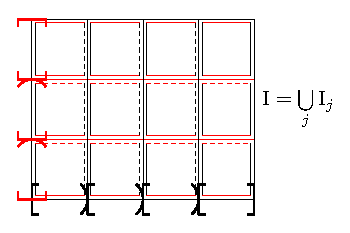
\includegraphics[width=0.35\textwidth]{MA4L1_5.eps}
		\caption{Разбиение бруска $\MI$ на попарно непересекающиеся бруски.}
		\label{4_5}
	\end{figure}
	Если разбиение на промежутке по ребрам это разбиение на попарно непересекющиеся, то естественно получившиеся промежутки, как их произведения, будут тоже попарно непересекающимися. Иначе, можно было бы найти наложение разбиения рёбер друг на друга, а это было бы противоречием.
	
	Выбираем произвольные точки $\xi_j^N \in \MI_j^N$ и рассмотрим функцию:
	$$
		f_N(x) = \ddsum{j}{}f\left(\xi_j^N\right){\cdot}\chi_{\MI_j^N}(x)
	$$
	Заметим, что $\ddsum{j}{}\chi_{\MI_j^N}(x) \equiv 1, \, \forall x \in \MI$, поскольку бруски $\MI_j^N$ не пересекаются и только один из индикаторов принимает единичное значение. Тогда оценим разность:
	$$
		|f(x) - f_N(x)| \leq \ddsum{j}{}\left|f(x) - f\left(\xi_j^N\right)\right|{\cdot}\chi_{\MI_j^N}(x)
	$$
	Мы знаем, что $f$ - равномерно непрерывна, поскольку брусок это компакт $\Rightarrow$ по теореме Кантора непрерывная функция на компакте - равномерно непрерывна, тогда:
	$$
		\forall \VE > 0, \, \exists \, N_0 \colon \forall N > N_0, \, \|x -y\| < \dfrac{1}{N} \Rightarrow |f(x) - f(y)| < \VE
	$$
	Поскольку диаметр: $\diam{\left(\MI_j^N\right)} < \tfrac{1}{N}$, то $\left\|x - \xi_j^N\right\| < \tfrac{1}{N}, \, \forall x \in \MI_j^N$, тогда:
	$$
		\ddsum{j}{}\left|f(x) - f\left(\xi_j^N\right)\right|{\cdot}\chi_{\MI_j^N}(x) \leq \ddsum{j}{}\VE{\cdot}\chi_{\MI_j^N}(x) = \VE{\cdot}\ddsum{j}{}\chi_{\MI_j^ N}(x) = \VE
	$$
	где неравенство верно в силу того, что $\left|f(x) - f\left(\xi_j^N\right)\right| < \VE$ для таких $x$ при которых $\chi_{\MI_j^N} \neq 0$. Тогда:
	$$
		f_N(x) \uconvm{\MI}{N \to \infty} f(x)
	$$ 
	Воспользовавшись теоремой, мы получаем требуемое.
\end{proof}
\begin{rem}
	Заметим, что все интегрируемые функции (даже в одномерном случае) не охватываются как равномерные пределы ступенчатых функций.
\end{rem}

\begin{exrc}
	Доказать, что $\chi_{\triangle 101}(x)$ интегрируема по Риману на $\MI$, но не приближается равномерно ступенчатыми функциями.
	\begin{figure}[H]
		\centering
		\includegraphics[width=0.2\textwidth]{MA4L1_6.png}
		\caption{Треугольник $\triangle 101$.}
		\label{4_6}
	\end{figure}
\end{exrc}
Суть проблемы в том, что наша ступенчатая функция составлена из индикаторов прямоугольников с рёбрами параллельными осям. 
\begin{proof}
	Пусть $\MJ = \triangle 101, \, \MI = [0,1]\times [0,1]$, тогда по доказанному выше:
	$$
		\ddint{\MI}{}\chi_{\triangle 101}(x)dx = |\MJ| = \dfrac{1}{2}{\cdot}1{\cdot}1 = \dfrac{1}{2}
	$$
	По аналогии со следствием выше разобъем $\MI$ на непересекающиеся бруски $\MI_j^N$, где $\diam\left(\MI_j^N\right) < \tfrac{1}{N}$, аналогично выбираем произвольные точки $\xi_j^N \in \MI_j^N$ и рассмативаем функцию:
	$$
		f_N(x) = \ddsum{j}{}\chi_{\triangle 101}\left(\xi_j^N\right){\cdot}\chi_{\MI_j^N}(x)
	$$
	Пусть $\MI_k^N$ - брусок, находящийся на диагонали $\triangle 101$. Оценим разность функций на нём: 
	$$
		\forall x \in \MI_k^N, \, |\chi_{\triangle 101}(x) - f_N(x)| = \left|\chi_{\triangle 101}(x) - \chi_{\triangle 101}\left(\xi_k^N\right)\right|
	$$
	тогда, если $\xi_k^N \in \triangle 101$, то можно взять $x \not\in \triangle 101$, а если $\xi_k^N \in \triangle 101$, то можно взять $x \in \triangle 101$. Следовательно, мы получаем следующую оценку:
	$$
		\sup\limits_{x \in \MI_k^N}\left|\chi_{\triangle 101}(x) - \chi_{\triangle 101}\left(\xi_k^N\right)\right| = 1 \not\to 0
	$$
	Следовательно, равномерной сходимости ступенчатых функций к $\chi_{\triangle 101}$ нет.
\end{proof}

Данный пример иллюстрирует, почему таких ступенчатых функций не хватает. В связи с этим появляется задача расширения класса интегрируемости. Как нам получить критерий интегрируемости?

\section*{Критерий интегрируемости}
\begin{theorem}
	Пусть $f$ - ограниченная функция на замкнутом бруске $\MI$. $f$ - интегрируема по Риману на $\MI$ тогда и только тогда, когда $\exists$ последовательности ступенчатых функций $h_n, g_n$ такие, что:
	\begin{enumerate}[label=\arabic*)]
		\item $h_n(x) \leq h_{n+1}(x); \,  g_{n+1}(x) \leq g_n(x),\, \forall n$;
		\item $h_n(x) \leq f(x) \leq g_n(x),\, \forall n$;
		\item $\ddint{\MI}{}g_n(x)dx - \ddint{\MI}{}h_n(x)dx \xrightarrow[n \to \infty]{} 0$;
	\end{enumerate}
\end{theorem}
\begin{rem}
	Отметим, что это фактически критерий Дарбу, изложенный на языке функций, где равномерная сходимость заменена на монотонную последовательность.
\end{rem}

\end{document}